
\documentclass[a4paper,12pt]{article}
\usepackage{../mypackages}
\usepackage{../macros}

\title{Chapitre XXX - Cours sur ...}
\author{N. Bancel}
\date{[[XXX MOIS ANNEE]]}


\begin{document}

\textbf{Collège Lycée Suger}
\hfill
\textbf{[[MATIERE]]} \\

\textbf{Année 2024-2025 - [[Numéro de]] trimestre}
\hfill
\textbf{[[CLASSE]]} \par

{\let\newpage\relax\maketitle}

%\begin{center}
%\textbf{\textcolor{red}{Infos importantes}} \\
%\end{center}

\begin{tcolorbox}[colback=blue!10!white, colframe=blue!75!black, title=Concepts importants à retenir]
  \begin{compactitem}
    \item Exo 1 page 17
    \item Exo 2 page 17
  \end{compactitem}
\end{tcolorbox}



\begin{figure}[H]
  \centering
  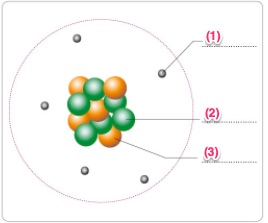
\includegraphics[width=0.4\linewidth]{img/atomes.png}
  \captionsetup{labelformat=empty}
  \caption{\label{} Blablabla}
\end{figure}


\end{document}
